\documentclass[uplatex]{jsarticle}
\usepackage{subfiles}
\usepackage{array,booktabs}
\usepackage{float}
\usepackage{amsmath}
\usepackage[dvipdfmx]{graphicx}
\usepackage[dvipdfmx,bookmarks=true]{hyperref}
\usepackage{pxjahyper}
\usepackage{ascmac}
\usepackage{siunitx}
\graphicspath{{images/}{../images/}}


\begin{document}


\title{先端人工知能論最終課題レポート}
\author{下村拓}
\date{2018/08/03}
\maketitle


\section{設定した問題の概要}
日本人、韓国人、中国人などはとても似た顔をしている。
しかし、我々日本人は微妙な違いを見分けかなりの精度でこれらの国を見分けることができる。
このタスクを機械が同様の精度で行うことができれば様々な場所で活躍できると考えられる。
例えば、液晶に映る日本語と外国語の表示切り替えを前に立っている外国人の数等で、
時間配分を変えることが可能であると考えている。
よって、今回は日本人か外国人かの判定をCNNに行わせることとする。


\section{利用した手法の概要と工夫点}
モデルのアーキテクチャとしては基本的にAlexNetのものを用いるところから始めた。
ただし、$50\times50$の画像を入力するため、次元数は異なる。

まずは画像データについて、正規化するために255で割ることで0から1の浮動小数点とした。
また、全ての画素値の平均と分散を求め、

\begin{equation}
  \frac{data - mean}{std}
\end{equation}

とすることで標準化を行った。

次にデータオーギュメンテーションを行った。
画像を水平に移動させるものと、画像を水平に反転させるものの二種類のデータ拡張の手法を用いた。

モデルについては、AlexNetをベースにしたが、
次元が減ることが不利になるのではないかと考え、MaxPooling層を削った。
Max Pooling層の代わりにConvolution層を増やした。
また、学習をしていく上で、常にヴァリデーションデータとトレインデータのロスの差が
大きかったことから、過学習を抑制できていないと考えられたため、
Dropoutの層を増やした。
最後の全結合については、データを単に平滑化すると重みの数が増えるため、
Global Average Polling層を用いて1次元データにした。

損失関数において外国人をミスした際に大きなペナルティが発生するように調整するべきであったが、
うまく実装できなかった。


\section{利用したデータ}
今回はJリーグ選手の顔を用いた。
理由は、外国人選手が含まれていることと一括で大量のラベル付き顔写真が得られるからである。
Jリーグ公式の選手名鑑から$50\times50$の画像と身長や体重、出身地の情報を取得した。
出身地の情報から日本の都道府県であるかないかで日本人と外国人のラベルをつけた。

データは全部で601件あり、日本人と外国人はそれぞれ516, 85件であった。
偏りがあるためダウンサンプリング、あるいはアッパーサンプリング、損失関数の重みづけを
するべきであったが、今回はデータ数が少ないためダウンサンプリングは避けたかったこと、
人の顔というセンシティブなものを扱うため、アッパーサンプリングも難しかったこと、
損失関数の重みづけがうまく実装できなかったことが重なり、偏ったままの学習となった。


\section{得られた結果と評価}
全データの7割を訓練用に、1割を検証用、2割をテスト用として扱った。
下表は最終的な訓練、検証、テストの精度、ロスを並べたものである。

\begin{table}[H]
  \caption{学習結果}
  \begin{center}
    \begin{tabular}{lc} \hline
      train accuracy & 0.2434 \\
      train loss & 0.9149 \\
      validation accuracy & 0.9375 \\
      validation loss & 0.1873 \\
      test accuracy & 0.2233 \\
      test loss & 0.9024 \\ \hline
    \end{tabular}
  \end{center}
\end{table}

テスト画像は123件あり、日本人が103件、外国人が20件存在した。
その中で誤ったテストは12件で日本人が4人、外国人が8人となっている。
上表の環境の下、テストで誤った画像を下に示す。

\begin{figure}[H]
  \begin{center}
    \includegraphics{../data/err_images/0.jpg}
    \includegraphics{../data/err_images/1.jpg}
    \includegraphics{../data/err_images/2.jpg}
    \includegraphics{../data/err_images/3.jpg}
    \includegraphics{../data/err_images/4.jpg}
    \includegraphics{../data/err_images/5.jpg}
    \\
    \includegraphics{../data/err_images/6.jpg}
    \includegraphics{../data/err_images/7.jpg}
    \includegraphics{../data/err_images/8.jpg}
    \includegraphics{../data/err_images/9.jpg}
    \includegraphics{../data/err_images/10.jpg}
    \includegraphics{../data/err_images/11.jpg}
    \caption{テストで誤った画像}
  \end{center}
\end{figure}

また、学習の進捗状況を数に示す。

\begin{figure}[H]
  \begin{center}
    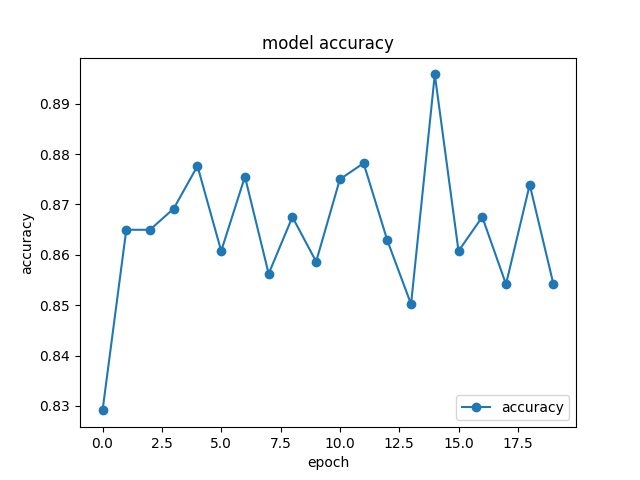
\includegraphics[width=7cm]{../data/history/acc.png}
    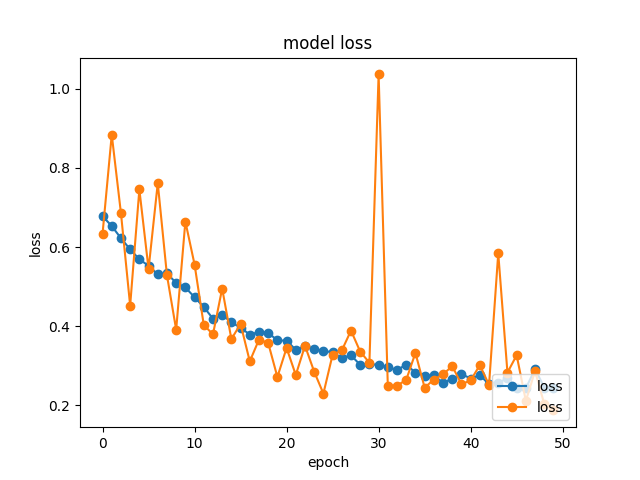
\includegraphics[width=7cm]{../data/history/loss.png}
    \caption{学習の進捗}
  \end{center}
\end{figure}

図からは学習がそれほどか学習せずに進んだことがわかる。
これはデータ拡張やDropout層を積んだことの成果であると考えられる。

精度は概ね9割となっているが、外国人選手が全体の役15\%であることや、
表からほとんど外国人の判定は行えていないことがわかる。
これは先述の通り、データの偏りがあることからほとんどの画像を日本人と判定するという
局所解にはまってしまったと考えられる。

本モデルを向上させるために続けてできる工夫は
\begin{itemize}
  \item データを増やす
  \item 外国人のデータを拡張する
  \item 損失関数において外国人を間違えた際に大きなペナルティを付与する
\end{itemize}

などが考えられる。


\end{document}
